\section{Available Hardware}

\subsection{Motor Controller}



\subsection{Motor and Propeller}
The quadrotor is equipped with four brushless outrunner motors named Turing Multistar. Bushless outrunners have in general more torque than inrunners, and can turn lager propellers, resulting in greater lift. The motors are controller by motorcontrollers, described in another section. The propeller comes with the motor. It is XX long and has a SHAPE (find proper name). 
The relationship between PWM signal to the motor controllers and the velocity of the propeller can be seen in Figure ZZ. 

\begin{figure}[H]
	\centering
	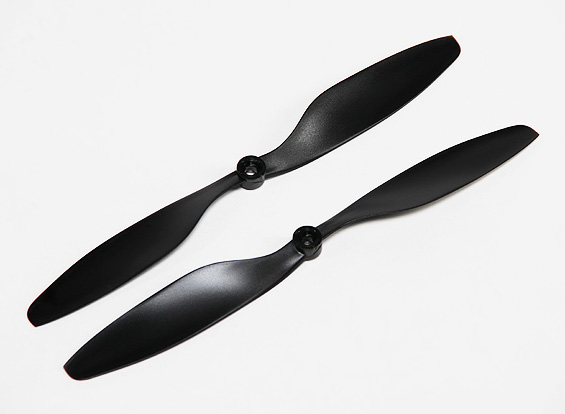
\includegraphics[scale=0.5]{figures/propeller.png}
	\caption{Two of the four propellers 										mounted on the quadrotor.[http://www.hobbyking.com/hobbyking/store/__58215__MT2213_935KV_MultiStar_Motor_and_Propeller_Combo_10x4_5_CW_CCW_EU_Warehouse_.html2 
]}
	\label{fig:Propeller}
\end{figure}
It has been observed during tests, that the motor runs faster as its temperature increases. This is not expected due to the increased resistance, that occurs when the coils within the motor are heated. Therefore the relationship between PWM signal and velocity is not representative for all cases. It is however deemed reasonable to neglect this variance and presume a relationship as it is derived in the measurement report, see Appendix YY. 
\newpar 
\begin{figure}[H]
	\centering
	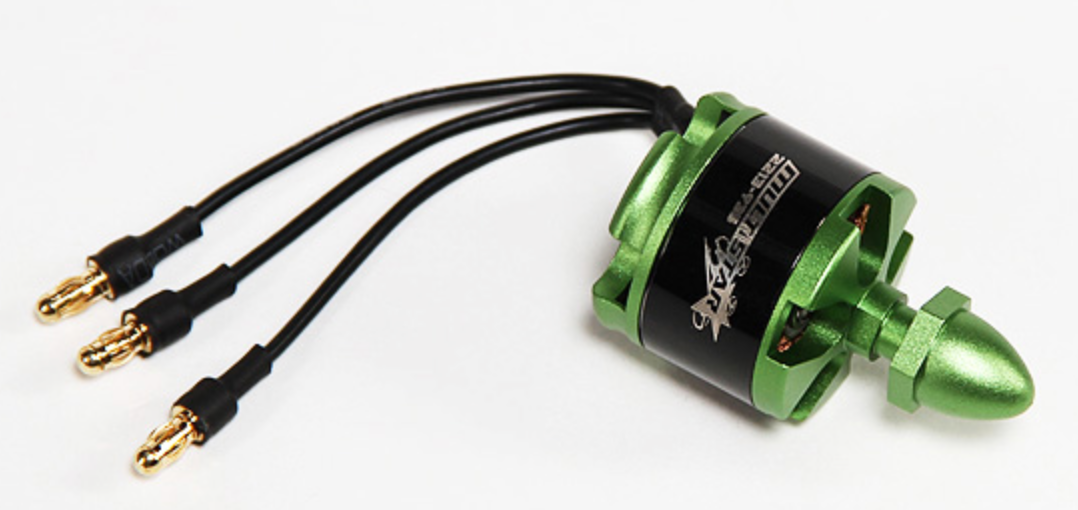
\includegraphics[scale=0.5]{figures/motor.png}
	\caption{One of the four motors mounted on the quadrotor.[http://www.hobbyking.com/hobbyking/store/__58215__MT2213_935KV_MultiStar_Motor_and_Propeller_Combo_10x4_5_CW_CCW_EU_Warehouse_.html2 
]}
	\label{fig:Motor}
\end{figure}


Moreover it shall be noted, that the battery level drops over time, with a significance, that can not be neglected, as it has great impact on the output of the motor and therefore on the lift of the propeller. It is possible to measure the battery level while operating the quadrotor. By taking into account the battery level in the test of the PWM signal to velocity, it is possible to obtain a quadcopter having constant lift force, if this is requested. 

\subsection{Platform}

\subsection{Battery}

The battery available for the prototype, is a Zippy Flightmax battery. Its weights 141 gram, has an capacity of 1500 mAh, a voltage of 11.1 volts and a discharge current of 20 amperes. 


\subsection{Vicon System}

The Vicon system is a powerful tool that provides real-time position and orientation data captured with NROFCAMERAS infrared cameras.This information can be used to track objects inside the room the system is built in. An example is found in Aalborg University as seen in \figref{ViconRoom}. 

%\begin{figure}[H]
%	\centering
%	\includegraphics[scale=0.5]{figures/ViconRoom}
%	\caption{Aalborg University's Vicon room.}
%	\label{ViconRoom}
%\end{figure}

For using this system, markers are attached to the object that is to be tracked. The Vicon system streams the position of the markers and the position and orientation of the object at 100 Hz for a computer to read them. The data can be received by using a SDK plugin for MATLAB. In this way, data can be operated in the MATLAB enviroment, making easier to obtain derived variables like velocities or accelerations.

The user interface of the Vicon system is shown in \figref{ViconTracker}. It is called Vicon Tracker and it allows the creation of objects by grouping markers present in the room. It also allows to change the center of gravity of the created objects and rotate the inertial and body reference frames to any desired orientation.
%\begin{figure}[H]
%	\centering
%	\includegraphics[scale=0.5]{figures/ViconTraker}
%	\caption{User interface of the Vicon System, the Vicon Tracker. An object has been created and its center of gravity is being modified.}
%	\label{ViconTracker}
%\end{figure}